% \input{mmd6-cpf-leader}
% ***Begin: mmd6-cpf-leader
%
%	Configure LaTeX to produce an article using the memoir class
%

\documentclass[12pt,oneside,oldfontcommands]{memoir}
\usepackage[absolute]{textpos}

% Setup CLARREO Pathfinder document
% \input{mmd6-cpf-setup}
% ***Begin: mmd6-cpf-setup
%
%	Generic Configuration for memoir-based documents
%

\usepackage{layouts}[2001/04/29]

% In case we need a glossary, or index
\usepackage[automake,acronyms,shortcuts,nopostdot,nonumberlist,nogroupskip]{glossaries}
\renewcommand{\glossarysection}[2][]{}
\setglossarystyle{longheader}
\renewcommand{\entryname}{Acronym}
\renewcommand{\descriptionname}{Complete Term}
\setlength{\glsdescwidth}{1\linewidth}
\glstoctrue
\makeglossaries
\makeindex

% Basic page layout configuration
\def\mychapterstyle{default}
\def\mypagestyle{headings}










% ***End: mmd6-cpf-setup

% Use 8.5 x 11 inch page layout
% \input{mmd6-cpf-layout-8.5x11}
% ***Begin: mmd6-cpf-layout-8.5x11
%
%	8.5 x 11 layout for CPF memoir-based documents
%


%%% need more space for ToC page numbers
\setpnumwidth{1.0em}
\setrmarg{3.55em}

%%% need more space for ToC section numbers
\cftsetindents{part}{0.5em}{3em}
\cftsetindents{chapter}{1.0em}{3em}
\cftsetindents{section}{3.0em}{4.25em}
\cftsetindents{subsection}{4.25em}{3.0em}
\cftsetindents{subsubsection}{8.4em}{4.8em}
\cftsetindents{paragraph}{10.7em}{5.7em}
\cftsetindents{subparagraph}{12.7em}{6.7em}

%%% need more space for LoF numbers
\cftsetindents{figure}{1.0em}{3.0em}

%%% and do the same for the LoT
\cftsetindents{table}{1.0em}{3.0em}

%%% set up the page layout
\settrimmedsize{\stockheight}{\stockwidth}{*}	% Use entire page
\settrims{0pt}{0pt}

\setlrmarginsandblock{1.5in}{1.5in}{*}
\setulmarginsandblock{1.5in}{1.5in}{*}
\setmarginnotes{17pt}{51pt}{\onelineskip}
\setheadfoot{2\onelineskip}{.4\onelineskip}
\setheaderspaces{*}{2\onelineskip}{*}
\checkandfixthelayout% ***End: mmd6-cpf-layout-8.5x11

% Use default packages for memoir, cdh, and CPF setup
% \input{mmd6-memoir-packages}
% ***Begin: mmd6-memoir-packages
%
%	Default packages for memoir documents created by MultiMarkdown
%

\usepackage{fancyvrb}			% Allow \verbatim et al. in footnotes
\usepackage{graphicx}			% To enable including graphics in pdf's
\usepackage{booktabs}			% Better tables
\usepackage{tabulary}			% Support longer table cells
\usepackage[T1]{fontenc}		% Use T1 font encoding for accented characters
\usepackage[utf8]{inputenc}		% For UTF-8 support
\usepackage{xcolor}				% Allow for color (annotations)
\usepackage{listings}			% Allow for source code highlighting
\usepackage[sort&compress]{natbib} % Better bibliography support

% \usepackage[normalem]{ulem}		% Support strikethrough

% \input{mmd6-criticmarkup}
% ***Begin: mmd6-criticmarkup
% CriticMarkup Support
\usepackage{soul}
\usepackage{xargs}
\usepackage{todonotes}
\newcommandx{\cmnote}[2][1=]{\todo[linecolor=red,backgroundcolor=red!25,bordercolor=red,#1]{#2}}

% ***End: mmd6-criticmarkup
% ***End: mmd6-memoir-packages
% \input{mmd6-cdh-packages}
% ***Begin: mmd6-cdh-packages
\let\footruleskip\undefined %undefine footruleskip

\usepackage{fancyhdr}
\usepackage{amsmath}
\usepackage{amssymb}
\usepackage[version=3]{mhchem}
\usepackage{lastpage}
\usepackage{mathabx}
\usepackage{mathrsfs}
\usepackage[margin=1.0in]{geometry}
\usepackage{siunitx}
\usepackage{enumitem}
\usepackage{lineno}
\usepackage{placeins}
\usepackage{pdflscape}
\usepackage{placeins}
\usepackage[normalem]{ulem}
\usepackage{ebgaramond}
\usepackage{longtable}
\usepackage{multicol}
\usepackage{microtype}
\usepackage{etoolbox}
\usepackage{footmisc}
\usepackage{fontspec}
\setsansfont{Helvetica}
\setmainfont{Times New Roman}
% \defaultfontfeatures{Ligatures=TeX}
% \setmainfont{EB Garamond}
% \fontspec[ItalicFont={EB Garamond 12 Italic}]
% \setmonofont{Inconsolata}
% \setmathsfont(Digits,Latin,Greek){TeX Gyre Termes}
% \renewcommand\emshape{\itshape}

% \usepackage{acronym}
% \usepackage{mathspec}
% \usepackage{caption}
% \usepackage{lscape}
% \usepackage[titletoc]{appendix}
% \usepackage[perpage,symbol*]{footmisc}
% \usepackage[symbol*]{footmisc}
% \usepackage{layouts}
% \usepackage{cleveref}
% \let\printglossary\relax
% \let\theglossary\relax
% \let\endtheglossary\relax
% \def\bibliostyle{chicago}
% \usepackage{wasysym}




% ***End: mmd6-cdh-packages
% \input{mmd6-cpf-packages}
% ***Begin: mmd6-cpf-packages
\usepackage[para,flushleft]{threeparttable}% ***End: mmd6-cpf-packages

% Configure default metadata to avoid errors
% \input{mmd6-default-metadata}
% ***Begin: mmd6-default-metadata
%
%	Configure default metadata in case it's missing to avoid errors
%

\def\myauthor{Author}
\def\defaultemail{}
\def\defaultposition{}
\def\defaultdepartment{}
\def\defaultaddress{}
\def\defaultphone{}
\def\defaultfax{}
\def\defaultweb{}
\def\defaultaffiliation{}

\def\mytitle{Title}
\def\subtitle{}
\def\mykeywords{}
% \def\keywords{}


\def\bibliostyle{plain}
% \def\bibliocommand{}

\def\myrecipient{}

% Overwrite with your own if desired
%\input{ftp-metadata}

% ***End: mmd6-default-metadata

% \input{mmd6-cpf-header-reformat}
% ***Begin: mmd6-cpf-header-reformat

%

% %
% % Define Page Styles
% %
% \pagestyle{fancy}
% \setlength\hoffset{-0.2in}
% \setlength\topmargin{-20pt}
% \setlength\textheight{600pt}
% \setlength\footskip{50pt}
% \renewcommand{\headrulewidth}{0.0pt}
% % Hard-coded title due to mutlicolumn error
% \lhead{\begin{tabular}[b]{|p{3.75in}|p{2.7in}|} \hline Revision:~\revision & Document No:~\documentnumber\\ \hline Release Date:~\releasedate&Page:~\thepage~of~\pageref{LastPage}\\ \hline \multicolumn{2}{|l|}{Title:~Mission Concept of Operations}\\ \hline \end{tabular}}
% % \lhead{\begin{tabular}[b]{|p{3.75in}|p{2.7in}|} \hline Revision:~\revision & Document No:~\documentnumber\\ \hline Release Date:~\releasedate&Page:~\thepage~of~\pageref{LastPage}\\ \hline \multicolumn{2}{|l|}{Title:~\mytitle}\\ \hline \end{tabular}}
% \chead{}
% % \chead{\mytitle}
% \rhead{}
% \cfoot{\scriptsize The electronic version is the offical approved document.\\Verify this is the correct version before use.}


% \fancypagestyle{firststyle}
% {
%    \fancyhf{}
%    \fancyfoot[C]{\scriptsize  The electronic version is the offical approved document.\\Verify this is the correct version before use.}
%    \setlength\topmargin{-40pt}
%    \setlength\footskip{-65pt}
% }
% %
% % End Define Page Styles
% %
% % CPF SMRD-specific page styles to enable compile-time modification of revision and footer
%
% Define Page Styles
%
\pagestyle{fancy}
\setlength\hoffset{-0.2in}
\setlength\topmargin{-20pt}
\setlength\textheight{600pt}
\setlength\footskip{50pt}
\renewcommand{\headrulewidth}{0.0pt}
% Hard-coded title due to mutlicolumn error
\lhead{\begin{tabular}[b]{|p{3.75in}|p{2.7in}|} \hline Revision:~\revision & Document No:~\documentnumber\\ \hline Release Date:~\releasedate&Page:~\thepage~of~\pageref{LastPage}\\ \hline \multicolumn{2}{|l|}{Title:~Science and Mission Requirements Document}\\ \hline \end{tabular}}
\chead{}
% \chead{\mytitle}
\rhead{}
\cfoot{\scriptsize The electronic version is the official approved document.\\The requirements are from a CORE database query dated: 13 April 2018.\\Verify this is the correct version before use.}


\fancypagestyle{firststyle}
{
   \fancyhf{}
   \fancyfoot[C]{\scriptsize  The electronic version is the official approved document.\\The requirements are from a CORE database query dated: 13 April 2018.\\Verify this is the correct version before use.}
   \setlength\topmargin{-40pt}
   \setlength\footskip{-65pt}
}
%
% End Define Page Styles
%

% ***Begin: mmd6-cpf-page-styles
%
% Define Page Styles
%
\pagestyle{fancy}
\setlength\hoffset{-0.2in}
\setlength\topmargin{-20pt}
\setlength\textheight{600pt}
\setlength\footskip{50pt}
\renewcommand{\headrulewidth}{0.0pt}
% Hard-coded title due to mutlicolumn error
\lhead{\begin{tabular}[b]{|p{3.75in}|p{2.7in}|} \hline Revision:~\revision & Document No:~\documentnumber\\ \hline Release Date:~\releasedate&Page:~\thepage~of~\pageref{LastPage}\\ \hline \multicolumn{2}{|l|}{Title:~Mission Concept of Operations}\\ \hline \end{tabular}}
\chead{}
% \chead{\mytitle}
\rhead{}
\cfoot{\scriptsize The electronic version is the official approved document.\\Verify this is the correct version before use.}


\fancypagestyle{firststyle}
{
   \fancyhf{}
   \fancyfoot[C]{\scriptsize  The electronic version is the official approved document.\\Verify this is the correct version before use.}
   \setlength\topmargin{-40pt}
   \setlength\footskip{-65pt}
}
%
% End Define Page Styles
%% ***End: mmd6-cpf-page-styles

% New Capitalize Macro
\makeatletter
\newcommand{\Capitalize}[1]{%
  \edef\@tempa{\expandafter\@gobble\string#1}%
  \edef\@tempb{\expandafter\@car\@tempa\@nil}%
  \edef\@tempa{\expandafter\@cdr\@tempa\@nil}%
  \uppercase\expandafter{\expandafter\def\expandafter\@tempb\expandafter{\@tempb}}%
  \@namedef{\@tempb\@tempa}{\expandafter\MakeUppercase\expandafter{#1}}}
\makeatother
% End New Capitalize Macro


\makeatletter
\let\ps@plain\ps@fancy
\makeatother

% Formatting of TOC

%
% Redefine document section hyperref labels
%
\def\subsubsectionautorefname{Section}
\def\subsectionautorefname{Section}
\def\sectionautorefname{Section}
\def\chapterautorefname{Section}
%
% Complete hyperref label redefinition
%

% \tightlists
\setlist{itemsep=.1mm, topsep=0mm}
\setlist[enumerate,1]{leftmargin=0.5cm}
\renewcommand{\theenumi}{\alph{enumi}}

% \renewcommand*{\afterlottitle}{\vspace{0em}}


%
% Define Chapter Styles
%
\makechapterstyle{cpf}{%
\setlength{\afterchapskip}{-0.5\baselineskip}
  \setlength{\beforechapskip}{\baselineskip}
  \setlength{\headsep}{2.0\baselineskip}
  \renewcommand*{\chapterheadstart}{}
  \renewcommand*{\printchaptername}{}
  \renewcommand*{\chapternamenum}{}
  \renewcommand*{\printchapternum}{\sffamily\large\bfseries\thechapter.0\space}
  \renewcommand*{\afterchapternum}{}
  \renewcommand{\printchaptertitle}[1]{%
    \raggedright{##1}}
}

\makechapterstyle{appendix}{%
  \setlength{\afterchapskip}{\baselineskip}
  \setlength{\beforechapskip}{\baselineskip}
  \setlength{\headsep}{2.0\baselineskip}
  \renewcommand*{\chapterheadstart}{}
  \renewcommand*{\printchaptername}{\sffamily\large\center\bfseries APPENDIX\space}
  \renewcommand*{\chapternamenum}{}
  \renewcommand*{\printchapternum}{\thechapter\space}
  \renewcommand*{\afterchapternum}{}
  \renewcommand{\printchaptertitle}[1]{%
    \center\bfseries{##1}}
}
%
% End Chapter Styles Definition
%

%
% Define Table Styles to enable bold first row
%
\newcolumntype{+}{>{\global\let\currentrowstyle\relax}}
\newcolumntype{^}{>{\currentrowstyle}}
\newcommand{\rowstyle}[1]{\gdef\currentrowstyle{#1}%
#1\ignorespaces
}
%
% End Table Style Definition
%


%
%
% Define Table of Contents, Figures, Tables, Appendices Formatting
%
\renewcommand{\contentsname}{\large\sffamily TABLE OF CONTENTS}
\renewcommand{\listfigurename}{\large\sffamily TABLE OF FIGURES}
\renewcommand{\cftfigurename}{Figure\space}
\renewcommand{\listtablename}{\large\sffamily TABLE OF TABLES}
\renewcommand{\cfttablename}{Table\space}
\renewcommand{\cftappendixname}{\normalsize Appendix\space}
\renewcommand{\cftchapteraftersnum}{.0}
\renewcommand{\cftchapterfont}{\normalfont}
\renewcommand{\cftchapterpagefont}{\normalfont}
\renewcommand{\cftsectionfont}{\normalsize}
\setlength{\cftbeforechapterskip}{0.0in}
\renewcommand{\cftchapterdotsep}{\cftdotsep}% Chapters should use dots in ToC
\renewcommand{\printtoctitle}[1]{\centering\Large\bfseries #1}
\renewcommand{\printloftitle}[1]{\centering\Large\bfseries #1}
\renewcommand{\printlottitle}[1]{\centering\Large\bfseries #1}
\renewcommand{\aftertoctitle}{%
	\par\nobreak\normalsize\bfseries\quad SECTION\mbox{}\hfill{PAGE}\par\nobreak}
\renewcommand{\afterlottitle}{%
	\par\nobreak}
\renewcommand{\afterloftitle}{%
	\par\nobreak}
\setcounter{tocdepth}{2}
% End Table of Contents, Figures, Tables, Appendices Formatting


%
% Define Table of Appendices
%
\cftinsertcode{preapp}{\setcounter{tocdepth}{-10}}
\newcommand\apptoc{
  \begingroup
  \cftinsertcode{prenorm}{\setcounter{tocdepth}{-10}}
  \cftinsertcode{preapp}{\setcounter{tocdepth}{0}}
  \renewcommand\contentsname{\large\sffamily TABLE OF APPENDICES}
  \renewcommand{\aftertoctitle}{\par}
  \renewcommand{\cftchapteraftersnum}{}
  \normalfamily
  \tableofcontents*
 \endgroup
}
%
% End Table of Appendices Definitions
%


%
% Section Heading Formatting
%
\makeatletter
\renewcommand\paragraph{\@startsection
 {paragraph}{4}{0mm}%
 {-\baselineskip}%
 {1.0\baselineskip}%
 {\sffamily\bfseries\normalsize}}%
\makeatother

\makeatletter
\renewcommand\subparagraph{\@startsection
 {subparagraph}{5}{0mm}%
 {-\baselineskip}%
 {1.0\baselineskip}%
 {\sffamily\bfseries\normalsize}}%
\makeatother

\setsecheadstyle{\bfseries\sffamily\raggedright}
\setsubsecheadstyle{\bfseries\sffamily\raggedright}
\setsubsubsecheadstyle{\bfseries\sffamily\raggedright}

%
% End Section Heading Formatting
%

\makeatletter
\let\ps@plain\ps@fancy
\makeatother
% ***End: mmd6-cpf-header-reformat
% ***End: mmd6-cpf-leader
\def\myauthor{Craig Hutchinson}
\def\mytitle{Science and Mission Requirements Document (SMRD)}
\def\mydate{16 April 2018}
\def\releasedate{TBD}
\def\documentnumber{CPF-02-011}
\def\titlepagerevision{REV. C}
\def\revision{C  }
\longnewglossaryentry{Beta}{name=Beta}{preliminary data product not yet ready for scientific journal publications.}

\longnewglossaryentry{Edition 1}{name=Edition 1}{

data product ready for scientific journal publication}

\longnewglossaryentry{International System of Units}{name=International System of Units}{

From the French le Système international d'unités abbreviated SI.}

\longnewglossaryentry{Level 0 Data Product}{name=Level 0 Data Product}{

Reconstructed, unprocessed instrument and payload data at full resolution, with any and all communications artifacts (e.g., synchronization frames, communications headers, duplicate data) removed.}

\longnewglossaryentry{Level 1A Data Product}{name=Level 1A Data Product}{

Reconstructed, unprocessed instrument data at full resolution, time--referenced, and annotated with ancillary information, including radiometric and geometric calibration coefficients and geo--referencing parameters (e.g., platform ephemeris) computed and appended but not applied to the Level 0 data}

\longnewglossaryentry{Level 1B Data Product}{name=Level 1B Data Product}{

Level 1A data processed to sensor units and geo--located.}

\longnewglossaryentry{National Aeronautics and Space Administration}{name=National Aeronautics and Space Administration}{

The agency of the United States government that is responsible for the nation's civilian space program and for aeronautics and aerospace research.}

\longnewglossaryentry{analysis}{name=analysis}{

the technical evaluation process of using techniques and tools such as mathematical models and computer simulation, historical\slash design\slash test data, and other quantitative assessments to calculate characteristics and verify specification compliance. Analysis is used to verify requirements compliance where established techniques are adequate to yield confidence or where testing is impractical.}

\longnewglossaryentry{collect}{name=collect}{

to acquire data}

\longnewglossaryentry{demonstration}{name=demonstration}{

the qualitative determination of compliance with requirements by observation during actual operation or simulation under preplanned conditions and guidelines.}

\longnewglossaryentry{inspection}{name=inspection}{

a physical measurement or visual evaluation of equipment and associated documentation. Inspection is used to verify construction features, drawing compliance, workmanship, and physical condition.}

\longnewglossaryentry{measure}{name=measure}{

to look at a target and collect the radiation}

\longnewglossaryentry{point}{name=point}{

to orient sensor towards a target}

\longnewglossaryentry{sample}{name=sample}{

to collect an ensemble of measurements}

\longnewglossaryentry{test}{name=test}{

an actual operation of equipment, normally instrumented, under simulated or flight equivalent conditions or the subjection of parts or equipment to specified environments to measure and record responses in a quantitative manner.}

\newacronym{ABI}{ABI}{Advanced Baseline Imager}

\newacronym{ADCO}{ADCO}{Attitude Determination and Control Officer}

\newacronym{AFRAM}{AFRAM}{Active Flight Releasable Attachment Mechanism}

\newacronym{AGRI}{AGRI}{Advanced Geosynchronous Radiation Imager}

\newacronym{ASDC}{ASDC}{Atmospheric Sciences Data Center}

\newacronym{ATBD}{ATBD}{Algorithm Theoretical Basis Document}

\newacronym{ATL}{ATL}{Attitude Timeline}

\newacronym{AVHRR}{AVHRR}{Advanced Very High Resolution Radiometer}

\newacronym{BAD}{BAD}{Broadcast Ancillary Data}

\newacronym{BASEPLATE}{BASEPLATE}{Beta, Attitude, Significant Event Planning Table}

\newacronym{CERES}{CERES}{Clouds and Earth's Radiant Energy System}

\newacronym{CLARREO}{CLARREO}{Climate Absolute Radiance and Refractivity Observatory}

\newacronym{COMS}{COMS}{Communication, Ocean, and Meteorological Satellite}

\newacronym{CPF}{CPF}{CLARREO Pathfinder}

\newacronym{CPOC}{CPOC}{CPF Payload Operations Center}

\newacronym{CPRSP}{CPRSP}{CLARREO Pathfinder Reflected Solar Payload}

\newacronym{CSDS}{CSDS}{CPF Science Data System}

\newacronym{CSTOL}{CSTOL}{Colorado System Test and Operations Language}

\newacronym{DAAC}{DAAC}{Distributed Active Archive Center}

\newacronym{DEWG}{DEWG}{Dynamic Events Working Group}

\newacronym{EOSDIS}{EOSDIS}{Earth Observing System Data and Information System}

\newacronym{ESDIS}{ESDIS}{Earth Science Data and Information System}

\newacronym{ELC}{ELC}{ExPRESS Logistics Carrier}

\newacronym{EOTP}{EOTP}{Enhanced ORU Temporary Platform}

\newacronym{EUMETSAT}{EUMETSAT}{European Organization for the Exploitation of Meteorological Satellites}

\newacronym{ExPA}{ExPA}{ExPRESS Pallet Adapter}

\newacronym{ExPRESS}{ExPRESS}{Expedite the Processing of Experiments to Space Station}

\newacronym{FC}{FC}{Flight Controller}

\newacronym{FD}{FD}{Flight Director}

\newacronym{FLAWS}{FLAWS}{Flight Anomaly Worksheet}

\newacronym{FPA}{FPA}{Focal Plane Array}

\newacronym{FPE}{FPE}{Focal Plane Electronics}

\newacronym{FOV}{FOV}{Field of View}

\newacronym{FRAM}{FRAM}{Flight Releasable Attach Mechanism}

\newacronym{FSW}{FSW}{Flight Software}

\newacronym{GEO}{GEO}{Geostationary Earth Orbit}

\newacronym{GOCI}{GOCI}{Geostationary Ocean Color Imager}

\newacronym{GOES}{GOES}{Geostationary Operational Environmental Satellite}

\newacronym{GRAWS}{GRAWS}{Ground Anomaly Worksheet}

\newacronym{GSFC}{GSFC}{Goddard Space Flight Center}

\newacronym{HFSS}{HFSS}{High-rate Fine Sun Sensor}

\newacronym{HOSC}{HOSC}{Huntsville Operations Support Center}

\newacronym{H&S}{H&S}{Health and Status}

\newacronym{HySICS}{HySICS}{HyperSpectral Imager for Climate Science}

\newacronym{HPS}{HPS}{HySICS Pointing System}

\newacronym{HVPS}{HVPS}{High Voltage Power Supply}

\newacronym{IC SIPS}{IC SIPS}{Inter-Calibration Science Investigator Processing System}

\newacronym{ICPP}{ICPP}{Inter-Calibration Planning and Processing element}

\newacronym{ICS}{ICS}{ISS Communications Services}

\newacronym{IT}{IT}{Information Technology}

\newacronym{IMU}{IMU}{Inertial Measurement Unit}

\newacronym{IRS}{IRS}{Indian Remote Sensing}

\newacronym{HISIE}{HISIE}{HySICS Instrument-Spacecraft Interface Electronics}

\newacronym{ISRO}{ISRO}{Indian Space Research Organization}

\newacronym{ISS}{ISS}{International Space Station}

\newacronym{JPSS}{JPSS}{Joint Polar Satellite System}

\newacronym{JSC}{JSC}{Johnson Space Center}

\newacronym{KARI}{KARI}{Korea Aerospace Research Institute}

\newacronym{KSC}{KSC}{Kennedy Space Center}

\newacronym{LAADS}{LAADS}{Level-1 and Atmosphere Archive and Distribution System}

\newacronym{LaRC}{LaRC}{Langley Research Center}

\newacronym{LASP}{LASP}{The University of Colorado Laboratory for Atmospheric and Space Physics}

\newacronym{LEO}{LEO}{Low Earth Orbit}

\newacronym{LPF}{LPF}{Launch Provider Facility}

\newacronym{MCC-H}{MCC-H}{Mission Control Center-Houston}

\newacronym{MODS}{MODS}{Mission Operations and Data Systems}

\newacronym{MSFC}{MSFC}{Marshall Space Flight Center}

\newacronym{MTG-I}{MTG-I}{Meteosat Third Generation-Imaging}

\newacronym{NATC}{NATC}{NASA Threaded Coupling}

\newacronym{NOAA}{NOAA}{National Oceanic and Atmospheric Administration}

\newacronym{NPP}{NPP}{National Polar-orbiting Partnership}

\newacronym{OASIS-CC}{OASIS-CC}{Operations and Science Instrument Support Command Control}

\newacronym{OASIS-PS}{OASIS-PS}{Operations and Science Instrument Support Planning and Scheduling}

\newacronym{OLI}{OLI}{Operational Land Imager}

\newacronym{ORU}{ORU}{Orbital Replacement Unit}

\newacronym{OTCM}{OTCM}{ORU Tool Changeout Mechanism}

\newacronym{PDL}{PDL}{Payload Data Library}

\newacronym{PFRAM}{PFRAM}{Passive Flight Releasable Attachment Mechanism}

\newacronym{PIA}{PIA}{Payload Integration Agreement}

\newacronym{POIC}{POIC}{Payload Operations Integration Center}

\newacronym{PRCU}{PRCU}{Payload Rack Checkout Unit}

\newacronym{PRT}{PRT}{Platinum Resistance Thermometer}

\newacronym{PRTs}{PRTs}{Platinum Resistance Thermometers}

\newacronym{RAPTR}{RAPTR}{Remote Advanced Payload Test Rig}

\newacronym{RBI}{RBI}{Radiation Budget Instrument}

\newacronym{RS}{RS}{Reflected Solar}

\newacronym{SAPP}{SAPP}{Space Asset Protection Program}

\newacronym{SDP}{SDP}{Science Data Processing}

\newacronym{SI}{SI}{Système Internationale}

\newacronym{SIM}{SIM}{Spectral Irradiance Monitor}

\newacronym{SMRD}{SMRD}{Science and Mission Requirements Document}

\newacronym{SPDM}{SPDM}{Special Purpose Dexterous Manipulator}

\newacronym{SSF}{SSF}{Single Satellite Footprint}

\newacronym{SSPF}{SSPF}{Space Station Processing Facility}

\newacronym{STK}{STK}{Systems Tool Kit}

\newacronym{SWIR}{SWIR}{Shortwave Infrared}

\newacronym{TDP}{TDP}{Telemetry Data Processing}

\newacronym{TDRSS}{TDRSS}{Tracking and Data Relay Satellite System}

\newacronym{TEA}{TEA}{Torque Equilibrium Attitude}

\newacronym{TIMs}{TIMs}{Technical Interchange Meetings}

\newacronym{TLE}{TLE}{Two-Line Element}

\newacronym{TLM}{TLM}{Telemetry}

\newacronym{TOPO}{TOPO}{Trajectory Operations Officer}

\newacronym{TQSM}{TQSM}{Telemetry Quality and System Monitoring}

\newacronym{TReK}{TReK}{Telescience Resource Kit}

\newacronym{TSIS}{TSIS}{Total and Spectral Solar Irradiance Sensor}

\newacronym{UDP}{UDP}{User Datagram Protocol}

\newacronym{USGS}{USGS}{United States Geological Survey}

\newacronym{VDC}{VDC}{Volts direct current}

\newacronym{VIIRS}{VIIRS}{Visible Infrared Imaging Radiometer Suite}

\newacronym{VNIR}{VNIR}{Visible Near Infrared}

\newacronym{VPN}{VPN}{Virtual Private Network}

\newacronym{WSTF}{WSTF}{White Sands Test Facility}

% \input{mmd6-cpf-begin}
% ***Begin: mmd6-cpf-begin
%
%	For setup that must follow metadata included in the document
%

%
%	Get ready for the actual document
%

\usepackage[
	plainpages=false,
	pdfpagelabels,
	pdftitle={\mytitle},
	pagebackref,
	pdfauthor={\myauthor},
	pdfkeywords={\mykeywords},
  	draft
	]{hyperref}

\usepackage{memhfixc}
\usepackage{cleveref}

\ifx\watermark\undefined
\else
  \usepackage{draftwatermark}
  \SetWatermarkText{\watermark}
  \SetWatermarkScale{1}
  \SetWatermarkColor[gray]{0.9}
\fi

% \input{mmd6-cpf-title}
% ***Begin: mmd6-cpf-title
%
%	Configure information from metadata for use in title
%

\def\headingtitle{\mytitle}

\ifx\latexauthor\undefined
\else
	\def\myauthor{\latexauthor}
\fi

\ifx\documentnumber\undefined
\else
	\def\mycpftitle{\Large\bfseries DOC~NUMBER~\documentnumber}
\fi

\ifx\titlepagerevision\undefined
	\def\titlepagerevision{\revision}
\fi

\ifx\mydate\undefined
\else
	\addtodef{\mycpftitle}{}{ \\ \MakeUppercase Release Date:~\mydate}
\fi

\addtodef{\mycpftitle}{}{\\ \Large
	Climate Absolute Radiance and Refractivity Observatory \\
	(CLARREO Pathfinder) \\
	\mytitle
}


\ifx\subtitle\undefined
\else
	\addtodef{\mytitle}{}{ \\ \subtitle}
\fi

\ifx\affiliation\undefined
\else
	\addtodef{\myauthor}{}{ \\ \affiliation}
\fi

\ifx\address\undefined
\else
	\addtodef{\myauthor}{}{ \\ \address}
\fi

\ifx\phone\undefined
\else
	\addtodef{\myauthor}{}{ \\ \phone}
\fi

\ifx\email\undefined
\else
	\addtodef{\myauthor}{}{ \\ \email}
\fi

\ifx\event\undefined
\else
	\date[\mydate]{\today}
\fi

% ***End: mmd6-cpf-title


\title{\mycpftitle}
\author{\myauthor}

\ifx\mydate\undefined
\else
  \date{\mydate}
\fi


\ifx\theme\undefined
\else
	\usetheme{\theme}
\fi

\begin{document}
\cftinserthook{toc}{prenorm}


\mainmatter
\VerbatimFootnotes


%
% Define Figure and Table Name Styles
%
\captionnamefont{\small\sffamily}
\captiontitlefont{\small\sffamily}
\counterwithin{figure}{section}
\renewcommand\thefigure{\thesection-\arabic{figure}} 
\counterwithin{table}{section}
\renewcommand\thetable{\thesection-\arabic{table}}
% \renewcommand{\figurename}{\sffamily Figure}
% \renewcommand{\tablename}{\sffamily Table}
%
% End Figure and Table Name Style Definitions
%

% \input{mmd6-cpf-front-matter}
% ***Begin: mmd6-cpf-front-matter
% Title Page

\thispagestyle{firststyle}
\sffamily
\setlength\voffset{-18pt}
\setlength{\floatsep}{10pt plus 1.0pt minus 2.0pt}
\vspace{-0.25in}
\begin{table}[h!]
  % \centering
  \begin{tabular}{ m{6.5cm} r }
    \begin{minipage}{4in}
      
\includegraphics[width=1.32in, height=1.12in]{meatball.png}\\
        \textsf{\noindent
        \footnotesize{National Aeronautics and\\
        \vspace{-5pt}Space Administration}
        }

    \end{minipage}
    &
    \begin{minipage}[t]{10cm}
    \vspace{0.3in}
    \sffamily
    \raggedleft\Large\bfseries \documentnumber\\
    \normalsize \MakeUppercase \titlepagerevision\\
    % \vspace{-0.6in}
    \raggedleft\bfseries
    RELEASE DATE:~\MakeTextUppercase\releasedate
    \end{minipage}
  \end{tabular}
\end{table}
\vspace{-0.3in}
\rule{\linewidth}{2.25pt}
~\\
~\\
\vspace{0.42in}
\centering
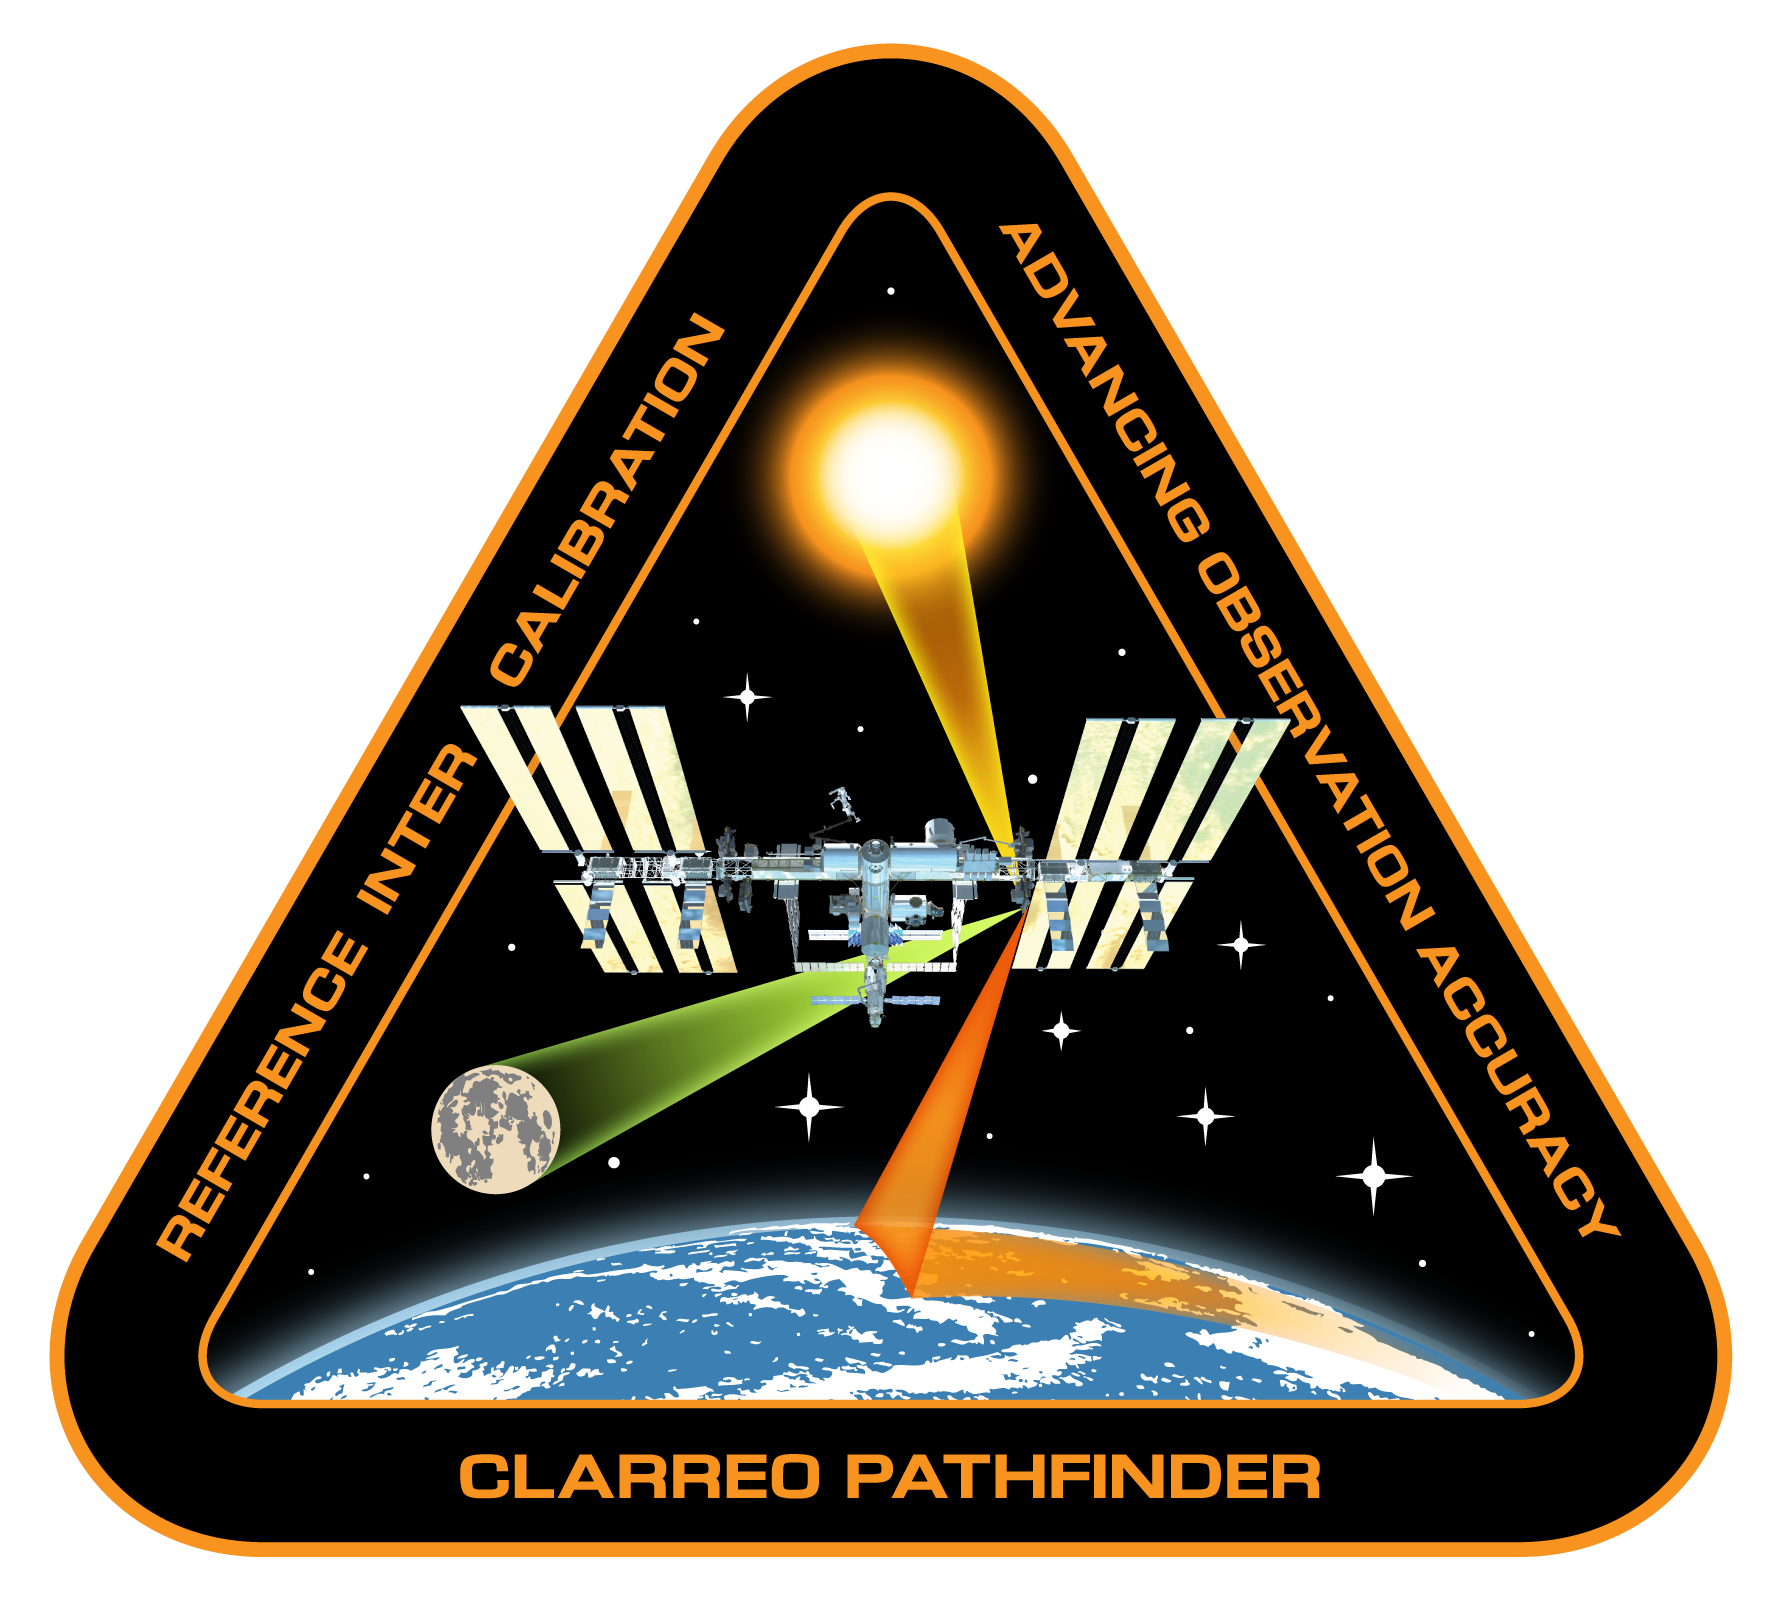
\includegraphics[keepaspectratio,width=2.3in]{cpf_logo.png}

\Large\bfseries
	Climate Absolute Radiance and Refractivity Observatory (CLARREO) Pathfinder \\
\vspace{0.4in}
\mytitle
\normalsize
\vspace{0.25in}
\mydate \\
\normalfont
\vspace{0.05in}
\fbox{
\begin{minipage}[t][9\height][c]{\dimexpr\textwidth-2\fboxsep-2\fboxrule\relax}
\centering
Approved for Public Release; Distribution is Unlimited
\end{minipage}
}
\clearpage

% Signature Page
% \bfseries
% \sffamily
% \center{\large SIGNATURE PAGE\par}
% \vspace{0.1in}
% \raggedright
% \normalfont
% \begin{table}[htbp]
% \begin{minipage}{\linewidth}
% \centering
% \small
% \begin{tabulary}{\textwidth}{p{3.325in}p{0.225in}p{2.5in}}
% \bfseries{~Prepared By:} & & \\[0.35in]
% \cmidrule(l){1-1}\cmidrule(l){3-3}
% ~Craig Hutchinson & & Tim Holden (LASP)\\
% ~Mission Architect & & Instrument Systems Engineer\\[0.25in]
% % \cmidrule(l){1-1}\cmidrule(l){3-3}
% % Name & & Name \\
% % Title & & Title \\[0.4in]
% \bfseries{~Concurred By:} & & \\[0.35in]
% \cmidrule(l){1-1}%\cmidrule(l){3-3}
% ~Jim Corliss & &  \\
% ~Science Manager & &  \\[0.35in]
% \cmidrule(l){1-1}%\cmidrule(l){3-3}
% ~Brian Boland & &  \\
% ~Systems Engineer & &  \\[0.35in]
% \cmidrule(l){1-1}%\cmidrule(l){3-3}
% ~Garfield Creary & &  \\
% ~Chief Engineer & &  \\[0.25in]
% \bfseries{~Approved By:} & & \\[0.35in]
% \cmidrule(l){1-1}%\cmidrule(l){3-3}
% ~Gary Fleming & &  \\
% ~Project Manager & &  \\[0.4in]
% % \cmidrule(l){1-1}\cmidrule(l){3-3}Name & & Name \\
% % Title & & Title \\[0.4in]
% \end{tabulary}
% \end{minipage}
% \end{table}
% \clearpage
% % Signature page for CLARREO Pathfinder SMRD
\bfseries
\sffamily
\center{\large SIGNATURE PAGE\par}
\vspace{0.1in}
\raggedright
\normalfont
\begin{table}[htbp]
\begin{minipage}{\linewidth}
\centering
\small
\begin{tabulary}{\textwidth}{p{3.325in}p{0.225in}p{2.5in}}
\bfseries{~Prepared By:} & & \\[0.35in]
~Electronic Approval on File\qquad\qquad\qquad2/21/2018\\
\cmidrule(l){1-1}%\cmidrule(l){3-3}
~Craig Hutchinson\\
~Systems Engineer\\[0.25in]
% \cmidrule(l){1-1}\cmidrule(l){3-3}
% Name & & Name \\
% Title & & Title \\[0.4in]
\bfseries{~Concurred By:} & & \\[0.35in]
~Electronic Approval on File\qquad\qquad\qquad3/1/2018\\
\cmidrule(l){1-1}%\cmidrule(l){3-3}
~Brian Boland & &  \\
~Lead Systems Engineer & &  \\[0.35in]
\bfseries{~Approved By:} & & \\[0.35in]
~Electronic Approval on File\qquad\qquad\qquad3/14/2018\\
\cmidrule(l){1-1}%\cmidrule(l){3-3}
~James Corliss & &  \\
~Chief Engineer & &  \\[0.35in]
~Electronic Approval on File\qquad\qquad\qquad2/27/2018\\
\cmidrule(l){1-1}%\cmidrule(l){3-3}
~Gary Fleming & &  \\
~Project Manager & &  \\[0.35in]
~Electronic Approval on File\qquad\qquad\qquad3/9/2018\\
\cmidrule(l){1-1}%\cmidrule(l){3-3}
~Bruce Wieliecki & &  \\
~Project Scientist & &  \\[0.4in]
% \cmidrule(l){1-1}\cmidrule(l){3-3}Name & & Name \\
% Title & & Title \\[0.4in]
\end{tabulary}
\end{minipage}
\end{table}
\clearpage
% ***Begin: sig_page
% Signature page for CLARREO Pathfinder SMRD
\bfseries
\sffamily
\center{\large SIGNATURE PAGE\par}
\vspace{0.1in}
\raggedright
\normalfont
\begin{table}[htbp]
\begin{minipage}{\linewidth}
\centering
\small
\begin{tabulary}{\textwidth}{p{3.325in}p{0.225in}p{2.5in}}
\bfseries{~Prepared By:} & & \\[0.35in]
% ~Electronic Approval on File\qquad\qquad\qquad2/21/2018\\
\cmidrule(l){1-1}%\cmidrule(l){3-3}
~Craig Hutchinson\\
~Systems Engineer\\[0.25in]
% \cmidrule(l){1-1}\cmidrule(l){3-3}
% Name & & Name \\
% Title & & Title \\[0.4in]
\bfseries{~Concurred By:} & & \\[0.35in]
% ~Electronic Approval on File\qquad\qquad\qquad3/1/2018\\
\cmidrule(l){1-1}%\cmidrule(l){3-3}
~Brian Boland & &  \\
~Lead Systems Engineer & &  \\[0.35in]
\bfseries{~Approved By:} & & \\[0.35in]
% ~Electronic Approval on File\qquad\qquad\qquad3/14/2018\\
\cmidrule(l){1-1}%\cmidrule(l){3-3}
~James Corliss & &  \\
~Chief Engineer & &  \\[0.35in]
% ~Electronic Approval on File\qquad\qquad\qquad2/27/2018\\
\cmidrule(l){1-1}%\cmidrule(l){3-3}
~Gary Fleming & &  \\
~Project Manager & &  \\[0.35in]
% ~Electronic Approval on File\qquad\qquad\qquad3/9/2018\\
\cmidrule(l){1-1}%\cmidrule(l){3-3}
~Bruce Wieliecki & &  \\
~Project Scientist & &  \\[0.4in]
% \cmidrule(l){1-1}\cmidrule(l){3-3}Name & & Name \\
% Title & & Title \\[0.4in]
\end{tabulary}
\end{minipage}
\end{table}
\clearpage% ***End: sig_page

% Revision History and TBX Table Page
% \sffamily
% \bfseries
% \center{\large REVISION HISTORY PAGE\par}
% \normalfont
% \centering
% \begin{table}[htbp]
% \begin{minipage}{\linewidth}
% \setlength{\tymax}{0.5\linewidth}
% \centering
% \small
% \begin{tabular}{| >{\centering\arraybackslash}m{1.25in}| >{\centering\arraybackslash}m{2.95in}| >{\centering\arraybackslash}m{1.5in}|} \hline
% \bfseries{Revision No.} & \bfseries{Description} & \bfseries{Release Date}\\
% \hline
% Preliminary & Mission Concept Review & N/A \\
% \hline
% \revision & System Requirements and Mission Definition Review & \releasedate \\
% \hline
% \end{tabular}
% % \end{tabulary}
% \end{minipage}
% \end{table}
% 
            \clearpage
            \sffamily
            \bfseries
            \center{\large TBX LIST\par}
            \normalfont
            \centering
            \begin{table}[htbp]
            \begin{minipage}{\linewidth}
            \setlength{\tymax}{0.5\linewidth}
            \centering
            \small\begin{tabular}{| >{\centering\arraybackslash}m{1.25in}| >{\centering\arraybackslash}m{2.95in}| >{\centering\arraybackslash}m{1.5in}|} \hline
            \bfseries{Item} & \bfseries{Description} & \bfseries{Page}\\
            \hline
            TBR & Delivery destination and role of PCU in CPRSP testing & \pageref{tbx_1}  \\ 
 \hline 
TBR & Pending thermal analysis of whether survival heaters are necessary for PCU & \pageref{tbx_2}  \\ 
 \hline 
TBR & Pending thermal analysis of whether there is thermal interface with Adaptor Plate & \pageref{tbx_3}  \\ 
 \hline 
TBR & Voltage of Discrete Input Signals & \pageref{tbx_4}  \\ 
 \hline 
TBR & Value of Bus A maximum current & \pageref{tbx_5}  \\ 
 \hline 
TBR & Value of Bus B maximum current & \pageref{tbx_6}  \\ 
 \hline 
TBR & Value of Bus C maximum current & \pageref{tbx_7}  \\ 
 \hline 
TBD & Drawing from LASP showing PCU positioning on ExPA & \pageref{tbx_8}  \\ 
 \hline 
TBD & Molecular Deposition onto Other Payloads Limit & \pageref{tbx_9}  \\ 
 \hline 
TBD & Molecular Deposition onto Other ISS Elements Limit & \pageref{tbx_10}  \\ 
 \hline 
TBD & Axial Launch Load Limit & \pageref{tbx_11}  \\ 
 \hline 
TBD & Lateral Launch Load Limit & \pageref{tbx_12}  \\ 
 \hline 
TBR & Minimum Natural Frequency & \pageref{tbx_13}  \\ 
 \hline 
TBD & Tolerance of thermal mass & \pageref{tbx_14}  \\ 
 \hline 
TBD & Thermal Testing Temperature & \pageref{tbx_15}  \\ 
 \hline 
\end{tabular}
        \end{minipage}
        \end{table}
        \raggedright
        \clearpage
% \clearpage
% % CLARREO Pathfinder SMRD Revision History and TBX Table Page for non-Supplemental document
\sffamily
\bfseries
\center{\large REVISION HISTORY PAGE\par}
\normalfont
\centering
\begin{table}[htbp]
\begin{minipage}{\linewidth}
\setlength{\tymax}{0.5\linewidth}
\centering
\small
\begin{tabular}{| >{\centering\arraybackslash}m{1.25in}| >{\centering\arraybackslash}m{2.95in}| >{\centering\arraybackslash}m{1.5in}|} \hline
\bfseries{Revision No.} & \bfseries{Description} & \bfseries{Release Date}\\
\hline
Baseline & Baseline. See CPF-CR-007 & 29 June 2017 \\
\hline
A & See CPF-CR-011 & 17 January 2018 \\
\hline
B & See CPF-CR-012 & 14 March 2018 \\
\hline
C & See CPF-CR-013 & \releasedate \\
\hline
\end{tabular}
% \end{tabulary}
\end{minipage}
\end{table}

            \clearpage
            \sffamily
            \bfseries
            \center{\large TBX LIST\par}
            \normalfont
            \centering
            \begin{table}[htbp]
            \begin{minipage}{\linewidth}
            \setlength{\tymax}{0.5\linewidth}
            \centering
            \small\begin{tabular}{| >{\centering\arraybackslash}m{1.25in}| >{\centering\arraybackslash}m{2.95in}| >{\centering\arraybackslash}m{1.5in}|} \hline
            \bfseries{Item} & \bfseries{Description} & \bfseries{Page}\\
            \hline
            TBR & Delivery destination and role of PCU in CPRSP testing & \pageref{tbx_1}  \\ 
 \hline 
TBR & Pending thermal analysis of whether survival heaters are necessary for PCU & \pageref{tbx_2}  \\ 
 \hline 
TBR & Pending thermal analysis of whether there is thermal interface with Adaptor Plate & \pageref{tbx_3}  \\ 
 \hline 
TBR & Voltage of Discrete Input Signals & \pageref{tbx_4}  \\ 
 \hline 
TBR & Value of Bus A maximum current & \pageref{tbx_5}  \\ 
 \hline 
TBR & Value of Bus B maximum current & \pageref{tbx_6}  \\ 
 \hline 
TBR & Value of Bus C maximum current & \pageref{tbx_7}  \\ 
 \hline 
TBD & Drawing from LASP showing PCU positioning on ExPA & \pageref{tbx_8}  \\ 
 \hline 
TBD & Molecular Deposition onto Other Payloads Limit & \pageref{tbx_9}  \\ 
 \hline 
TBD & Molecular Deposition onto Other ISS Elements Limit & \pageref{tbx_10}  \\ 
 \hline 
TBD & Axial Launch Load Limit & \pageref{tbx_11}  \\ 
 \hline 
TBD & Lateral Launch Load Limit & \pageref{tbx_12}  \\ 
 \hline 
TBR & Minimum Natural Frequency & \pageref{tbx_13}  \\ 
 \hline 
TBD & Tolerance of thermal mass & \pageref{tbx_14}  \\ 
 \hline 
TBD & Thermal Testing Temperature & \pageref{tbx_15}  \\ 
 \hline 
\end{tabular}
        \end{minipage}
        \end{table}
        \raggedright
        \clearpage
\clearpage

% ***Begin: rev_hist_compile
% CLARREO Pathfinder SMRD Revision History and TBX Table Page for Supplemental document
\sffamily
\bfseries
\center{\large REVISION HISTORY PAGE\par}
\normalfont
\centering
\begin{table}[htbp]
\begin{minipage}{\linewidth}
\setlength{\tymax}{0.5\linewidth}
\centering
\small
\begin{tabular}{| >{\centering\arraybackslash}m{1.25in}| >{\centering\arraybackslash}m{2.95in}| >{\centering\arraybackslash}m{1.5in}|} \hline
\bfseries{Revision No.} & \bfseries{Description} & \bfseries{Release Date}\\
\hline
Baseline Supplemental& Baselinewith supplemental information. Rationale and verification information is included. See CPF-CR-007 & 29 June 2017 \\
\hline
A Supplemental& See CPF-CR-011 & 17 January 2018 \\
\hline
B Supplemental & See CPF-CR-012 & 14 March 2018 \\
\hline
\revision & See CPF-CR-013 & \releasedate \\
\hline
\end{tabular}
% \end{tabulary}
\end{minipage}
\end{table}
% 
            \clearpage
            \sffamily
            \bfseries
            \center{\large TBX LIST\par}
            \normalfont
            \centering
            \begin{table}[htbp]
            \begin{minipage}{\linewidth}
            \setlength{\tymax}{0.5\linewidth}
            \centering
            \small\begin{tabular}{| >{\centering\arraybackslash}m{1.25in}| >{\centering\arraybackslash}m{2.95in}| >{\centering\arraybackslash}m{1.5in}|} \hline
            \bfseries{Item} & \bfseries{Description} & \bfseries{Page}\\
            \hline
            TBR & Delivery destination and role of PCU in CPRSP testing & \pageref{tbx_1}  \\ 
 \hline 
TBR & Pending thermal analysis of whether survival heaters are necessary for PCU & \pageref{tbx_2}  \\ 
 \hline 
TBR & Pending thermal analysis of whether there is thermal interface with Adaptor Plate & \pageref{tbx_3}  \\ 
 \hline 
TBR & Voltage of Discrete Input Signals & \pageref{tbx_4}  \\ 
 \hline 
TBR & Value of Bus A maximum current & \pageref{tbx_5}  \\ 
 \hline 
TBR & Value of Bus B maximum current & \pageref{tbx_6}  \\ 
 \hline 
TBR & Value of Bus C maximum current & \pageref{tbx_7}  \\ 
 \hline 
TBD & Drawing from LASP showing PCU positioning on ExPA & \pageref{tbx_8}  \\ 
 \hline 
TBD & Molecular Deposition onto Other Payloads Limit & \pageref{tbx_9}  \\ 
 \hline 
TBD & Molecular Deposition onto Other ISS Elements Limit & \pageref{tbx_10}  \\ 
 \hline 
TBD & Axial Launch Load Limit & \pageref{tbx_11}  \\ 
 \hline 
TBD & Lateral Launch Load Limit & \pageref{tbx_12}  \\ 
 \hline 
TBR & Minimum Natural Frequency & \pageref{tbx_13}  \\ 
 \hline 
TBD & Tolerance of thermal mass & \pageref{tbx_14}  \\ 
 \hline 
TBD & Thermal Testing Temperature & \pageref{tbx_15}  \\ 
 \hline 
\end{tabular}
        \end{minipage}
        \end{table}
        \raggedright
        \clearpage
% ***Begin: tbx_table

            \clearpage
            \sffamily
            \bfseries
            \center{\large TBX LIST\par}
            \normalfont
            \centering
            \begin{table}[htbp]
            \begin{minipage}{\linewidth}
            \setlength{\tymax}{0.5\linewidth}
            \centering
            \small\begin{tabular}{| >{\centering\arraybackslash}m{1.25in}| >{\centering\arraybackslash}m{2.95in}| >{\centering\arraybackslash}m{1.5in}|} \hline
            \bfseries{Item} & \bfseries{Description} & \bfseries{Page}\\
            \hline
            TBD & Expected POIC to CPOC interface requirements document & \pageref{tbx_1}  \\ 
 \hline 
TBD & Launch Vehicle Requirement Originator & \pageref{tbx_2}  \\ 
 \hline 
\end{tabular}
        \end{minipage}
        \end{table}
        \raggedright
        \clearpage% ***End: tbx_table
\clearpage% ***End: rev_hist_compile

\glsunsetall
\normalfont
\setlength{\beforechapskip}{-16pt}
\setcounter{tocdepth}{5}
\tableofcontents*
\setlength{\beforechapskip}{6pt}
\apptoc
\listoftables*
\listoffigures*
\glsresetall
\clearpage

\setcounter{secnumdepth}{5}
\setlist[enumerate,1]{label=\arabic*., ref=\arabic*}

\raggedright
\setlength{\parskip}{\baselineskip}
\chapterstyle{cpf}% ***End: mmd6-cpf-front-matter
% % List of acronyms that tend to be nested. This enables LaTeX to reliably expand acronyms
\newacronym{OTCM}{OTCM}{\gls{ORU} Tool Changeout Mechanism}
\newacronym{EOTP}{EOTP}{Enhanced \gls{ORU} Temporary Platform}
% ***Begin: nestedacros
% List of acronyms that tend to be nested. This enables LaTeX to reliably expand acronyms
\newacronym{OTCM}{OTCM}{\gls{ORU} Tool Changeout Mechanism}
\newacronym{EOTP}{EOTP}{Enhanced \gls{ORU} Temporary Platform}% ***End: nestedacros




% ***End: mmd6-cpf-begin

\chapter{Introduction }
\label{introduction}

\section{Purpose and Scope }
\label{purposeandscope}

This document establishes the \gls{CLARREO} Pathfinder science and mission requirements, which are derived from the Program-Level Requirements for the \gls{CPF} Project and captured in the Earth Systematic Missions Program Plan, Appendix Z.

\section{Document Organization }
\label{documentorganization}

\autoref{sec_docs} lists applicable and reference documents. \autoref{sec_desc} provides an overview of the \gls{CPF} science objectives and mission segments. \autoref{sec_req} contains the science and mission requirements. Appendices A and B provide acronyms and definitions.

\chapter{Documents  }
\label{sec_docs}

This section identifies documents that are applicable to this document and assumes the current version unless otherwise noted. Reference documents are for information only.

\section{Applicable Documents }
\label{applicabledocuments}


% Double vertical bar above is kludge to get around python code bug


\begin{table}[htbp]
\begin{minipage}{\linewidth}
\setlength{\tymax}{0.5\linewidth}
\centering
\small
\begin{tabulary}{\textwidth}{|+p{1.8in}|^p{4.2in}|} \hline
\rowstyle{\bfseries}%
 Document Number & Document Title \\
\hline

 420--01--01 & Earth Systematic Missions Program Plan, Appendix Z -- \gls{CLARREO} Pathfinder Program Level Requirements \\
 \gls{CPF}--01--013 & \gls{CLARREO} Pathfinder Statement of Work \\
 \gls{CPF}--02--002 & \gls{CLARREO} Pathfinder Systems Engineering Management Plan \\
 \gls{CPF}--02--009 & \gls{CLARREO} Pathfinder Mission Concept of Operations \\
 \gls{CPF}--03--001 & \gls{CLARREO} Pathfinder Mission Assurance Requirements \\
 SSP 51700 & Payload Safety Policy and Requirements for the International Space Station \\
 SSP 57003 & External Payload Interface Requirements Document \\
\hline

\end{tabulary}
\end{minipage}
\end{table}

\section{Reference Documents }
\label{referencedocuments}


% Double vertical bar above is kludge to get around python code bug


\begin{table}[htbp]
\begin{minipage}{\linewidth}
\setlength{\tymax}{0.5\linewidth}
\centering
\small
\begin{tabulary}{\textwidth}{|+p{1.8in}|^p{4.2in}|} \hline
\rowstyle{\bfseries}%
 Document Number & Document Title \\
\hline

 152--TP--003--003 & Glossary of Terms for the \gls{EOSDIS} Core System Project \\
 \gls{CPF}--04--014 & \gls{CLARREO} Pathfinder Data Management Plan \\
 \gls{GSFC}--423--SPEC--001 & NASA Earth Science Data Preservation Content Specification \\
 Lukashin et al, IEEE 2013 & Uncertainty Estimates for Imager Reference Inter--calibration with \gls{CLARREO} Reflected Solar Spectrometer \\
 NASA SP--2016--6105 Rev 2 & NASA Systems Engineering Handbook \\
 NPR 7120.5 & NASA Space Flight Program and Project Management \\
 NPR 7123.1 & NASA Systems Engineering Processes and Requirements \\
 PIP--16--039 & Payload Interface Agreement for \gls{CLARREO} Pathfinder \\
 Wielicki et al, IGA\gls{RS} 2008 & Climate Quality Broadband and Narrowband Solar Reflected Radiance Calibration Between Sensors in Orbit \\
 Wu et al, IEEE 2015 & Sensitivity of inter--calibration uncertainty of the \gls{CLARREO} reflected solar spectrometer features \\
\hline

\end{tabulary}
\end{minipage}
\end{table}

\section{Document Control }
\label{documentcontrol}

This document is managed by the \gls{CPF} Project and, after initial approval, will be placed under configuration control using the change management processes defined in the \gls{CLARREO} Pathfinder Configuration Management Operating Procedure (CPF-01--005).

\section{Order of Precedence }
\label{orderofprecedence}

The Program-Level Requirements and Project-Level plans listed in the applicable documents section take precedence over the \gls{SMRD}. The \gls{SMRD} takes precedence over all lower level requirement documents. Nothing in this document, however, supersedes applicable laws and regulations.

\chapter{System Description  }
\label{sec_desc}

This section describes the highest three levels of system architecture for the \gls{CPF} mission and provides context for requirements in \autoref{sec_req}. Refer to \gls{CLARREO} Pathfinder Mission Concept of Operations, \gls{CPF}-02--009, for a more thorough description of the mission functions and operations as well as details of lower levels in the architectural hierarchy.

\section{Mission Description }
\label{missiondescription}

\gls{CLARREO} is a Tier 1 mission recommended by the 2007 National Research Council Decadal Survey entitled ``Earth Science and Applications from Space: National Imperatives for the Next Decade and Beyond.'' The foundation of \gls{CLARREO} is the ability to produce highly accurate climate records to \gls{test} climate projections in order to improve models and enable sound policy decisions. The \gls{CLARREO} mission accomplishes this critical objective through accurate \gls{SI}-traceable decadal observations that are sensitive to many of the key climate parameters such as radiative forcings, climate responses, and feedbacks. Uncertainties in these parameters drive uncertainty in current climate model projections. In 2016, the \gls{CLARREO} Project received funding for a Pathfinder mission to demonstrate essential \gls{measure}ment technologies for the \gls{RS} portions of the \gls{CLARREO} Tier 1 Decadal survey mission, to include on-orbit high accuracy \gls{SI}-traceable calibration and the ability to transfer that calibration to other on-orbit assets. The appropriated funds support the flight of an \gls{RS} spectrometer hosted on the \gls{ISS} in the calendar year 2022 time frame. Prime mission operations on \gls{ISS} are planned for one year, with an additional year of data \gls{analysis} support following the end of the prime mission.

\gls{CPF} is a NASA-directed mission executed under the direction of the Science Mission Directorate – Earth Science Division. \gls{CPF} is a Category 3 mission per NPR 7120.5E and a Class D payload risk classification per NPR 8705.4. The mission has two baseline mission objectives:

\begin{enumerate}
\item{} Demonstrate the ability to conduct on-orbit, \gls{SI}-traceable calibration of \gls{measure}d scene spectral reflectance, with an advance in accuracy over current on-orbit sensors; and

\item{} Demonstrate the ability to use that improved accuracy to serve as an in orbit reference spectrometer for advanced inter-calibration of other key satellite sensors across most of the reflected solar spectrum (350 – 2300 nm).

\end{enumerate}

The \gls{CPF} will advance the accuracy and inter-calibration of satellite sensors. New techniques and technologies, that when applied on future missions, can reduce the time, relative to the use of existing space-based observations of reflected solar wavelengths, needed to detect climate change trends using reflected solar earth remote sensing observations. It also serves to reduce the uncertainty in societally critical research areas such as climate sensitivity and cloud feedback.

\section{Science Objectives }
\label{scienceobjectives}

The \gls{CPF} science objectives, as defined in section 4.1.1 of the PRLA, are the following:

\begin{enumerate}
\item{} Spectrally Resolved Earth Reflectance: The \gls{CPF} objective is to acquire on-orbit \gls{SI}-traceable spectrally resolved Earth reflectances referenced to spectral solar irradiance with average uncertainty <= 0.3\% (k=1) for the 350 - 2300 nm wavelength range.

\item{} Spectrally Integrated Earth Reflectance: The \gls{CPF} objective is to acquire on-orbit \gls{SI}-traceable broadband (350 - 2300 nm) spectrally-integrated Earth reflectance with uncertainty <= 0.3\% (k=1), with spectral accuracy weighted using global average Earth spectrally reflected energy.

\item{} On-Orbit Reference Inter-Calibration: The \gls{CPF} objective is to demonstrate the ability to use the reflected solar spectrometer as an in-orbit transfer standard for intercalibration of the reflectance bands of the \gls{VIIRS} instrument and the \gls{CERES} or \gls{RBI} instruments' shortwave channel. The inter-calibration uncertainties should be equal to or less than the spectrometer calibration uncertainties listed above.

\end{enumerate}

\section{System Architecture }
\label{systemarchitecture}

The \gls{CPF} Project system architecture is composed of the four mission segments required to successfully \gls{measure}, \gls{collect}, analyze, and distribute the \gls{CPF} science data. The \gls{CPF} mission segments, as shown in \autoref{cpf_arc} below and described in later sections are the Space Segment, Science Segment, Ground Segment, and Launch Segment. \gls{LASP} is responsible for elements shown in yellow, while \gls{LaRC} is responsible for elements shown in green. Elements shown in orange are external to the Project.

\begin{figure}[htbp]
\centering
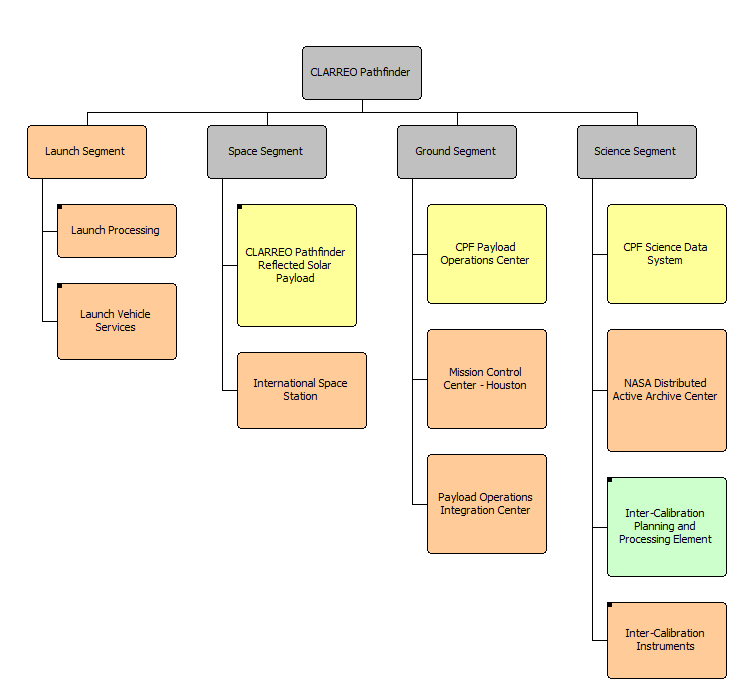
\includegraphics[keepaspectratio,width=\textwidth,height=8.5in]{20180416_cpf_architecture_l1-3.png}
\caption{\gls{CPF} System Architecture}
\label{cpf_arc}
\end{figure}

\section{Segment Definition }
\label{segmentdefinition}

\subsection{Space Segment }
\label{spacesegment}

The Space Segment is that portion of the architecture that flies in space and maintains the communication links between space and ground. It comprises the \gls{CPRSP} and the \gls{ISS}. The \gls{CPRSP} makes radiometric observations and transmits that information to the \gls{CPOC} via its attachment to the \gls{ISS}. The \gls{ISS} comprises the orbiting Space Station, all of its crew, visiting vehicles, attached non-\gls{CLARREO} Pathfinder payloads, and associated communications systems.

\subsection{Science Segment }
\label{sciencesegment}

The Science Segment includes all of the systems and facilities required to process, analyze (including calibration and validation of data), archive, and distribute the \gls{CPF} science data and data products. The Science Segment consists of four elements: the \gls{CSDS} at \gls{LASP}, a NASA \gls{DAAC}, the \gls{ICPP} element at \gls{LaRC}, and the Inter-Calibration Instruments. The Inter-Calibration Instruments are those specified by the On-Orbit Reference Inter-Calibration science objective. The NASA \gls{DAAC} will make the data products listed in the Standard Science Data Products table publicly available in accordance with NASA Earth Science Data and Information Policy with no period of exclusive access.

\subsection{Ground Segment }
\label{groundsegment}

The Ground Segment is the portion of the ground-based architecture that does not generate science products, and its primary role is to provide the monitoring, command, and control of the \gls{CPRSP}. It also processes and forwards the data received from the Space Segment to the Science Segment. It comprises the \gls{CPOC} at \gls{LASP}, \gls{MCC-H} at \gls{JSC}, and the \gls{POIC} at \gls{MSFC}.

\subsection{Launch Segment }
\label{launchsegment}

The Launch Segment is responsible for preparing the \gls{CPRSP} for flight and delivering it to the \gls{ISS}. The Launch Processing portion of the architecture prepares the \gls{CPRSP}, having completed final integration at \gls{KSC}, to function as an \gls{ISS} external payload. Launch Vehicle Services is the portion of the architecture responsible for transporting the \gls{CPRSP} from the Earth to the International Space Station. At this time, the identity of the Launch Vehicle Services provider and their associated requirements are not yet determined.

\chapter{Requirements  }
\label{sec_req}

\renewcommand\labelitemi{}

This section contains technical requirements, which define either what \gls{CPF} must do or a quality that the \gls{CPF} must have. Science Requirements trace directly to PLRA Baseline Science Requirements and specify performance of the overall \gls{CPF} mission. Mission Requirements allocate the \gls{SMRD} Science Requirements and PLRA Mission and Flight Element Performance Requirements to the Project-managed elements. The \gls{SMRD} groups Mission Requirements by segment.

The \gls{SMRD} distinguishes among requirements, goals, and statements of facts as follows:

\begin{itemize}
\item{} Shall: Used to indicate a binding requirement that will be verified

\item{} Should\slash May: Used to indicate a desired goal

\item{} Will: Used to indicate a statement of fact that the government will complete

\end{itemize}

The \gls{SMRD} allocates all Mission Requirements containing a ``shall'' to \gls{LASP}-managed elements. Goals are non-binding, while statements of fact are binding in that an expectation of certainty is established. Goals are included to guide trade studies and will be addressed at design reviews and technical interchange meetings. Values in this document listed as TBD or TBR are pending confirmation.

\section{Science Requirements}
\label{sciencerequirements}

\textbf{[CPF.20004]} Spectrally Resolved Earth Reflectance

The \gls{CLARREO} Pathfinder shall acquire on-orbit \gls{SI}-traceable spectrally resolved Earth reflectances referenced to spectral solar irradiance with average uncertainty <= 0.3\% (k=1) for the 350 - 2300 nm wavelength range.

\textbf{[CPF.20005]} Broadband Earth Reflectance

The \gls{CLARREO} Pathfinder shall acquire on-orbit \gls{SI}-traceable broadband reflectance (350 - 2300 nm) of Earth scenes with uncertainty <= 0.3\% (k=1).

\textbf{[CPF.20050]} Inter-Calibration Samples

The \gls{CLARREO} Pathfinder shall \gls{collect} inter-calibration sampling with \gls{CERES} or \gls{RBI} and \gls{VIIRS} sufficient to limit uncertainty contribution within 1 year of operations as specified in requirements \gls{CPF}.20004 and \gls{CPF}.20005.

\section{Mission Requirements}
\label{missionrequirements}

\subsection{Space Segment Requirements}
\label{spacesegmentrequirements}

\textbf{[RS.21000]} Wavelength

The \gls{CPRSP} shall \gls{measure} over the wavelength range of 350--2300 nm.

\textbf{[RS.21004]} Spectrally Resolved Earth Reflectance

The \gls{CPRSP} shall acquire on-orbit \gls{SI}-traceable spectrally resolved Earth reflectances referenced to spectral solar irradiance with average uncertainty <= 0.3\% (k=1) for the 350 - 2300 nm wavelength range.

\textbf{[RS.21005]} Broadband Earth Reflectance

The \gls{CPRSP} shall acquire on-orbit \gls{SI}-traceable broadband reflectance (350 - 2300 nm) of Earth scenes with uncertainty <= 0.3\% (k=1).

\textbf{[RS.21010]} Pointing Accuracy for Instrument Calibration

The \gls{CPRSP} shall have the ability to perform \gls{point}ing operations viewing Sun and Moon with sufficient accuracy to achieve uncertainty requirements \gls{RS}.21004 and \gls{RS}.21005.

\textbf{[RS.21011]} Angular Matching for Inter-Calibration

The \gls{CPRSP} shall perform Inter-Calibration sampling by directing the \gls{HySICS} Instrument boresight to within 0.7 degree (k=1) of a time-varying direction that is determined by the line of sight from the Inter-Calibration Instrument (at some instant of time consistent with the temporal matching requirement) to the \gls{HySICS} Instrument.

\textbf{[RS.21012]} Temporal Matching for Inter-Calibration

The \gls{CPRSP} shall perform inter-calibration operations viewing Earth within 10 minutes of \gls{LEO} Inter-Calibration Instruments (CERES\slash RBI and VIIRS) data acquisition events.

\textbf{[RS.21015]} Spectral Sampling

The \gls{CPRSP} shall \gls{sample} at a spectral precision of 3 nm or finer, equivalent to a 6 nm full width half maximum Gaussian bandwidth.

\textbf{[RS.21020]} Single Spectrum Precision for Inter-Calibration

The \gls{CPRSP} shall have a single spectrum precision of <= 3\% (k=1) relative to reflectance of 0.3 at solar zenith angle = 75 degrees. (This precision is at the scale of a single instantaneous 0.5 km field of view.)

\textbf{[RS.21025]} Along-track \gls{FOV}

The \gls{CPRSP} shall \gls{measure} \gls{RS} radiation continuously along-track with a field of view less than or equal to 0.5 km at nadir.

\textbf{[RS.21030]} Along-track Ground Sampling Distance

The \gls{CPRSP} shall \gls{measure} \gls{RS} radiation continuously along-track with a ground-sampling distance less than or equal to 0.5 km at nadir.

\textbf{[RS.21031]} Cross-track Ground Sampling Distance

The \gls{CPRSP} shall \gls{measure} \gls{RS} radiation continuously cross-track with a ground-sampling distance less than or equal to 0.5 km at nadir.

\textbf{[RS.21035]} Instrument Sensitivity to Polarization

The \gls{CPRSP} shall \gls{measure} the \gls{RS} radiation in the reflected solar spectra as a reference calibration to relevant climate sensors with polarization sensitivity less than 1\% (k=1) in wavelength range from 350 - 1800 nm and less than 2\% (k=1) from 1800 - 2300nm.

\textbf{[RS.21040]} Prime Mission Operations Period

The \gls{CPRSP} shall operate over a prime mission operation period of 1 year following commissioning activities.

\textbf{[RS.21041]} On-Orbit Commissioning Period

The \gls{CPRSP} shall complete commissioning activities within 60 days of installation to the \gls{ISS}.

\textbf{[RS.21045]} Decommissioning

The \gls{CPRSP} shall be capable of completing decommissioning activities within three months following the end of the science mission.

\textbf{[RS.21055]} Inter-Calibration Swath Width

The \gls{CPRSP} shall be capable of aiming the instrument boresight to match the full \gls{CERES}, \gls{RBI}, and \gls{VIIRS} instrument swath width (plus or minus 55°) when not obscured by \gls{ISS} structure.

\textbf{[RS.21060]} Geolocation of Earth-View Data

The \gls{CPRSP} shall have sufficient \gls{point}ing knowledge such that the \gls{CSDS} can determine the Earth viewing pixel geolocation to within 250 m (k=1) nadir equivalent.

\textbf{[RS.21110]} Swath Width

The \gls{CPRSP} shall \gls{measure} \gls{RS} radiation with a cross-track width greater than or equal to 70 km when centered at nadir.

\textbf{[RS.21150]} Inter-Calibration Operations

The \gls{CPRSP} shall be capable of performing 1 Inter-Calibration operation per orbit. An Inter-Calibration operation is defined as one of the following:

\begin{itemize}
\item{} - Measurement of spectral reflectance over entire lunar disk

\item{} - Inter-Calibration of space-borne instruments in low Earth orbit (LEO)

\item{} - Inter-Calibration of space-borne instruments in geostationary Earth orbit (GEO)

\end{itemize}

\textbf{[RS.22000]} Compliance with Launch Vehicle Requirements

The \gls{CPRSP} shall satisfy the launch vehicle requirements.

\textbf{[RS.22005]} Compliance with \gls{ISS} Requirements

The \gls{CPRSP} shall satisfy \gls{ISS} requirements.

\textbf{[RS.22010]} Compliance with Payload Interface Agreement Resource Allocations

The \gls{CPRSP} shall meet the resource allocations documented within the \gls{CPF} to \gls{ISS} \gls{PIA}.

\textbf{[RS.22025]} Measurements and Data Routing

The \gls{CPRSP} shall send science \gls{measure}ments and data to the \gls{CPOC}.

\textbf{[RS.22035]} Response to Ground Commands

The \gls{CPRSP} shall have the capability to accept ground commands.

\textbf{[RS.22040]} On-orbit Reprogramming

The \gls{CPRSP} shall have the capability of being reprogrammed while on orbit.

\subsection{Science Segment Requirements}
\label{sciencesegmentrequirements}

\subsubsection{Science Segment Requirements - LASP}
\label{sciencesegmentrequirements-lasp}

\textbf{[SCI.24000]} Data Product Delivery

The \gls{CSDS} shall deliver all Level 0 and Level 1B data products to the NASA \gls{DAAC} within the timelines specified for each data product in the Standard Science Data Products table.


\begin{table}[htbp]
\begin{minipage}{\linewidth}
\setlength{\tymax}{0.5\linewidth}
\centering
\small
\caption{Standard Science Data Products}
\label{tbl_std_sci_data_prod}
\begin{threeparttable}
\begin{tabulary}{\textwidth}{|+p{1.0in}|^p{3.0in}|^p{0.75in}|^p{0.75in}|} \hline
\rowstyle{\bfseries}%
\rowstyle{\bfseries}%
 Data Product & Description                                                         & First Data Delivery after IOC & Maximum data latency after first release\tnote{1} \\
\hline
 Level 0   & Reconstructed, unprocessed instrument and payload data at full resolution, with any and all communications artifacts (e.g., synchronization frames, communications headers, duplicate data) removed.           & 4 months       & 48 hours         \\
 Level 1B  & Calibrated and geolocated observations at full resolution, annotated with ancillary information such as radiometric and geometric calibration coefficients and georeferencing parameters (e.g., platform ephemeris).       & 8 months       & 1 month         \\
 Level 4   & Time\slash angle\slash space matched inter--calibration data for reference (CPF) and target sensors (CERES or RBI and VIIRS), scene information from target sensors (CERES or RBI and VIIRS), modeled parameters for estimated polarization and radiometric corrections. & 10 months      & 6 months         \\
\hline
\end{tabulary}
\begin{tablenotes}
\item[1] Data latency is defined as the elapsed time from the downlink to the availability of processed data products to the public.
\end{tablenotes}
\end{threeparttable}
\end{minipage}
\end{table}


\textbf{[SCI.24015]} Public Release of Data

The \gls{CSDS} shall make the Level 0 and Level 1B data listed in the Standard Science Data Products table, along with the scientific source code for algorithm software, coefficients, and ancillary data used to generate these products publicly available conforming to the NASA Earth Science Data and Information Policy (http:\slash \slash science.nasa.gov\slash earth-science\slash earth-science-data\slash data-information-policy\slash ).

\textbf{[SCI.24017]} Science Data Product Formats

The \gls{CSDS} shall format all Level 1B data products to conform to the HDF5 standard.

\textbf{[SCI.24018]} Long Term Knowledge Preservation

The \gls{CSDS} shall transfer to the NASA \gls{DAAC} all the information and documentation required for long-term preservation of knowledge about the Level 0 and Level 1B data products as defined in the NASA Earth Science Data Preservation Content Specification document published at http:\slash \slash earthdata.nasa.gov\slash about-eosdis\slash requirements.

\textbf{[SCI.24020]} Mission Lifetime - \gls{LASP}

The \gls{CSDS} shall be designed to support 60 days of commissioning, a prime mission operation period of 1 year, and 1 year of science post processing following the prime mission operation period.

\textbf{[SCI.24031]} Post Processing Geolocation for Earth-View Data

The \gls{CSDS} shall determine the geolocation of the Earth viewing pixels within 250 m (k=1) nadir equivalent.

\textbf{[SCI.24035]} Data Latency

The \gls{CSDS} shall deliver all required data to the NASA \gls{DAAC} within the timeframe specified in the Standard Science Data Products table.

\textbf{[SCI.24040]} \gls{ESDIS} Compliance

The \gls{CSDS} shall generate Level 0 and Level 1B data products whose metadata conform to ISO 19115 Geographic Information - Metadata standards and adhere to the Metadata Requirements --- Base Reference for NASA Earth Science Data Products document published at http:\slash \slash earthdata.nasa.gov\slash about-eosdis\slash requirements.

\textbf{[SCI.24050]} Full Resolution Browse Products

The \gls{CSDS} shall deliver to the NASA \gls{DAAC} full-resolution browse products for all science data.

\subsubsection{Science Segment Requirements - LaRC}
\label{sciencesegmentrequirements-larc}

\textbf{[SCI.24100]} Data Product Delivery

The \gls{ICPP} will deliver all Level 4 data products to the NASA \gls{DAAC} within the timelines specified for first data delivery associated with each data product in the Standard Science Data Products table.

\textbf{[SCI.24115]} Public Release of Data

The \gls{ICPP} will make the Level 4 data listed in the Standard Science Data Products table, along with the scientific source code for algorithm software, coefficients, and ancillary data used to generate these products publicly available conforming to the NASA Earth Science Data and Information Policy (http:\slash \slash science.nasa.gov\slash earth-science\slash earth-science-data\slash data-information-policy\slash ).

\textbf{[SCI.24117]} Science Data Product Formats

The \gls{ICPP} will format all Level 4 data products to conform to the HDF5 standard.

\textbf{[SCI.24118]} Long Term Knowledge Preservation

The \gls{ICPP} will transfer to the NASA \gls{DAAC} all the information and documentation required for long-term preservation of knowledge about the Level 4 data products as defined in the NASA Earth Science Data Preservation Content Specification document published at http:\slash \slash earthdata.nasa.gov\slash about-eosdis\slash requirements.

\textbf{[SCI.24120]} Mission Lifetime - \gls{LaRC}

The \gls{ICPP} will be designed to support 60 days of commissioning, a prime mission operation period of 1 year, and 1 year of science post processing following the prime mission operation period.

\textbf{[SCI.24126]} Inter-Calibration Planning

The \gls{ICPP} will provide the inter-calibration planning data to the \gls{CPOC} according to the \gls{CPOC} interface control document.

\textbf{[SCI.24130]} Inter-Calibrate Science Data

The \gls{ICPP} will inter-calibrate \gls{CLARREO} Pathfinder science data with \gls{VIIRS}.

\textbf{[SCI.24131]} Inter-Calibrate Science Data

The \gls{ICPP} will inter-calibrate \gls{CLARREO} Pathfinder science data with \gls{CERES}\slash \gls{RBI}.

\textbf{[SCI.24140]} \gls{ESDIS} Compliance

The \gls{ICPP} will generate Level 4 data products whose metadata conform to ISO 19115 Geographic Information - Metadata standards and adhere to the Metadata Requirements --- Base Reference for NASA Earth Science Data Products document published at http:\slash \slash earthdata.nasa.gov\slash about-eosdis\slash requirements.

\subsection{Ground Segment Requirements}
\label{groundsegmentrequirements}

\textbf{[GS.23000]} \gls{POIC} Interface

The \gls{CPOC} shall interface with the \gls{ISS} \gls{POIC} in accordance with the \gls{CPOC} to \gls{POIC} ICD (TBD).

\label{tbx_1}

\textbf{[GS.23005]} Generate Instrument Commanding

The \gls{CPOC} shall generate instrument commands and command loads for the execution of all \gls{CPRSP} functions on orbit.

\textbf{[GS.23010]} Transfer Command Information

The \gls{CPOC} shall transfer commands and command loads to the \gls{POIC} for upload to the \gls{ISS}.

\textbf{[GS.23015]} Validate Commands and Command Loads

The \gls{CPOC} shall validate commands and command loads prior to sending them to the \gls{POIC} for uploading to the \gls{CPRSP}.

\textbf{[GS.23020]} Generate Instrument Software Loads

The \gls{CPOC} shall generate instrument software loads to support \gls{CPRSP} operations.

\textbf{[GS.23030]} Health Maintenance of the Space Segment

The \gls{CPOC} shall monitor the health and safety of the \gls{CPRSP} and generate advisories of potentially unsafe conditions.

\textbf{[GS.23035]} Science Event Measurement Planning

The \gls{CPOC} shall have the capability of planning \gls{CPRSP} flight operations.

\textbf{[GS.23040]} Prime Mission Operational Lifetime

The \gls{CPOC} shall be designed to operate over a prime mission operation period of 1 year following commissioning activities.

\textbf{[GS.23045]} On-orbit Commissioning Period

The \gls{CPOC} shall complete \gls{CPRSP} commissioning activities within 60 days of installation to the \gls{ISS}.

\textbf{[GS.23050]} Data Processing

The \gls{CPOC} shall be designed to receive and process all science, H\&S, and ancillary data delivered from the \gls{ISS}.

\textbf{[GS.23055]} Data Storage

The \gls{CPOC} shall store \gls{CLARREO} Pathfinder data received from the \gls{ISS} until it has been successfully transferred to the \gls{DAAC}.

\textbf{[GS.23060]} Inter-Calibration Prioritization

The \gls{CPOC} shall command the \gls{CPRSP} to execute a sufficient number of inter-calibration events to meet the performance \gls{measure}s specified in \gls{CPF}.20050.

\subsection{Launch Segment Requirements}
\label{launchsegmentrequirements}

The launch vehicle is provided by the \gls{ISS} Program Office, and requirements for the launch vehicle are outside the scope of the \gls{CPF} system. Requirements levied from the launch vehicle originate from TBD\label{tbx_2} and are allocated to each segment, element, and subsystem directly through the allocations made by \gls{LASP}.


\begin{appendices}
\cftinserthook{toc}{preapp}
\chapterstyle{appendix}


\chapter{Acronyms and Abbreviations  }
\label{sec_acros}

\printglossary[type=\acronymtype]

\chapter{Glossary  }
\label{sec_gls}


\renewcommand{\entryname}{Term}
\renewcommand{\descriptionname}{Definition}
\printglossary


\end{appendices}

% \input{mmd6-cpf-footer}
% ***Begin: mmd6-cpf-footer
%
%	MultiMarkdown default footer file
%


% Back Matter
\if@mainmatter
	we're in main
	\backmatter
\fi


% Bibliography

\ifx\bibliocommand\undefined
\else
	\bibliographystyle{\bibliostyle}
	\bibliocommand
\fi



% Glossary
% \printglossaries


% Index
% \printindex

% ***End: mmd6-cpf-footer

\end{document}
